%%%%%%%%%%%%%%%%%%%%%%%%%%%%%%%%%%%%%%%%%%%%%%%%%%%%%%%%%
%                          导言区                        %
%%%%%%%%%%%%%%%%%%%%%%%%%%%%%%%%%%%%%%%%%%%%%%%%%%%%%%%%%
\documentclass[13pt]{ctexart} % 文档类
% 基础样式
\usepackage{geometry} % 设置页面
\renewcommand{\figurename}{Figure} % 设置标题 重命名为英文
\renewcommand{\tablename}{Table}
\renewcommand{\contentsname}{Contents}
\usepackage{changepage} % 设置摘要页缩减
\usepackage{fontspec} % 便于修改字体
\usepackage{fancyhdr} % 设置页眉页脚
\pagestyle{fancy} % 清空页眉页脚
\usepackage{lastpage}
\usepackage{titlesec} % 设置修改默认的section标题样式
\titleformat*{\section}{\LARGE\bfseries}
\titleformat*{\subsection}{\Large\bfseries}
\titleformat*{\subsubsection}{\Large\bfseries}
\usepackage[section]{placeins} % 新增: 浮动体不越过section
% 浮动体样式
\usepackage[shortlabels]{enumitem} % 设置列表缩进
\usepackage{booktabs} % 三线表宏包
\usepackage{array} % 设置表格的列格式
\usepackage{graphicx} % 插图片
\graphicspath{{C:/Users/zheng/Desktop/mcm-2021/mcmdocs/figs/}}
\usepackage{float} % 浮动体宏包 可禁用浮动效果
% 数学样式
\usepackage{amsmath} % 使用数学宏包
\usepackage{amsfonts} % 使用数学字体
% bib样式
\usepackage{etoolbox} % 设置参考文献不输出默认名
\usepackage{newtxtext}
\patchcmd{\thebibliography}{\section*{\refname}}{}{}{} % 引入网站作为参考文献
\usepackage[]{hyperref} % 设置引用且末尾不显示文档名
% 代码样式
\usepackage{url} % 设置等宽的代码字体
%%\setmonofont{IBM Plex Mono}
%% 建议这个,但我系统没这个字体,且懒得折腾了
%%windows用户请
\setmonofont{Courier New}
% 颜色
\usepackage{xcolor} % 代码高亮方案宏包
\usepackage{listings}
\definecolor{CPPLight}  {HTML} {686868}
\definecolor{CPPSteel}  {HTML} {888888}
\definecolor{CPPDark}   {HTML} {262626}
\definecolor{CPPBlue}   {HTML} {4172A3}
\definecolor{CPPGreen}  {HTML} {487818}
\definecolor{CPPBrown}  {HTML} {A07040}
\definecolor{CPPRed}    {HTML} {AD4D3A}
\definecolor{CPPViolet} {HTML} {7040A0}
\definecolor{CPPGray}   {HTML} {B8B8B8}
\lstset{
	basicstyle=\ttfamily,
	breaklines=true,
	framextopmargin=50pt,
	frame=bottomline,
	columns=fixed,
    %numbers=left,                                       % 在左侧显示行号
	frame=none,                                          % 不显示背景边框
	backgroundcolor=\color[RGB]{255,255,255},            % 设定背景颜色
	keywordstyle=\color[RGB]{40,40,255},                 % 设定关键字颜色
	numberstyle=\footnotesize\color{darkgray},           % 设定行号格式
	commentstyle=\itshape\color[RGB]{0,96,96},           % 设置代码注释的格式
	stringstyle=\slshape\color[RGB]{128,0,0},            % 设置字符串格式
	showstringspaces=false,                              % 不显示字符串中的空格
	language=python,                                     % 设置语言
	morekeywords={alignas,continute,friend,register,true,alignof,decltype,goto,
		reinterpret_cast,try,asm,defult,if,return,typedef,auto,delete,inline,short,
		typeid,bool,do,int,signed,typename,break,double,long,sizeof,union,case,
		dynamic_cast,mutable,static,unsigned,catch,else,namespace,static_assert,using,
		char,enum,new,static_cast,virtual,char16_t,char32_t,explict,noexcept,struct,
		void,export,nullptr,switch,volatile,class,extern,operator,template,wchar_t,
		const,false,private,this,while,constexpr,float,protected,thread_local,
		const_cast,for,public,throw,std},
	emph={map,set,multimap,multiset,unordered_map,unordered_set,numpy,graph,path,append,extend,
		unordered_multiset,unordered_multimap,vector,string,list,deque,
		array,stack,forwared_list,iostream,memory,shared_ptr,unique_ptr,
		random,bitset,ostream,istream,cout,cin,endl,move,default_random_engine,
		uniform_int_distribution,iterator,algorithm,functional,bing,numeric,},
	emphstyle=\color{CPPViolet},
}

%%%%%%%%%%%%%%%%%%%%%%%%%%%%%%%%%%%%%%%%%%%%%%%%%%%%%%%%%
%                         正文区                         %
%%%%%%%%%%%%%%%%%%%%%%%%%%%%%%%%%%%%%%%%%%%%%%%%%%%%%%%%%
\begin{document}
%%%%%%%%%%%%%%%%%%%%%%%%%%扉页%%%%%%%%%%%%%%%%%%%%%%%%%%
\newgeometry{left=1in,right=0.75in,top=1in,bottom=1in}
% 第一页的字体为times new roman
\setmainfont{Times New Roman}
\thispagestyle{empty}
% 扉页抬头

\vspace*{-16ex}
\centerline{\begin{tabular}{*3{c}}
        \parbox[t]{0.3\linewidth}{
            \begin{center}\textbf{Problem Chosen}\\ \Large \textcolor{red}{B}\end{center}
        }
         & \parbox[t]{0.3\linewidth}{\begin{center}\textbf{2021\\ MCM/ICM\\ Summary Sheet}\end{center}}
         & \parbox[t]{0.3\linewidth}{\begin{center}\textbf{Team Control Number}\\ \Large \textcolor{red}{2120710}\end{center}} \\\hline
    \end{tabular}}

\vspace*{3ex}

% 大标题
{\centering\fontsize{18}{16}\selectfont\textbf{{Fighting Wildfire with Unmanned Aerial Vehicles}}

    % summary
    \vspace{10pt}
    \fontsize{13}{10}\selectfont\textbf{{Summary}}\par}
\vspace{10pt}

% summray正文
\fontsize{13}{12.5}\selectfont %summary正文字体 13 pt
\begin{adjustwidth}{1cm}{1cm}
    \indent { }{ }{ }{ }{ }{ }
    In this research, we developed three models to simulate the use of Unmanned Aerial Vehicle in fighting fires. We use a hexagon coordinate system to modelize the region, and apply multi-factor evaluation to represent the landscape condition of the region. We also visualize the result to have a straight forward understanding to the situation.

    We use a Nervous System Model to describe the drones monitoring system. We use dynamic planning to sort out the solution: the least amount of SSA drones and repeater drones needed is $36$ and $96$.

    We use Drone-Terrian model to design the optimal hovering positions for drones in different terrains,we also visualize the result to give out the best hovering strategy.


    % 关键词
    \vspace{15pt}
    \textbf{key words} : Dynamic planning; Hexagonal coordinate system; Bushfire; Drones
\end{adjustwidth}

% 设置正文字体与geometry
\setmainfont[
    BoldFont       = texgyrepagella-bold.otf ,
    ItalicFont     = texgyrepagella-italic.otf ,
    BoldItalicFont = texgyrepagella-bolditalic.otf ]{texgyrepagella-regular.otf}
\newgeometry{left = 3.5cm, right = 3.5cm}

%%%%%%%%%%%%%%%%%%%%%%%%%%目录页%%%%%%%%%%%%%%%%%%%%%%%%%%
\newpage
\thispagestyle{empty}
\tableofcontents
%%%%%%%%%%%%%%%%%%%%%%%%%%正文页%%%%%%%%%%%%%%%%%%%%%%%%%%
\newpage
% 目录页后面是第一页
\setcounter{page}{1}

% 开始写正文
% 设置正文的页边距
\newgeometry{top=3cm, left=3.5cm, right=3.5cm}
% 设置正文的页眉页脚
\fancyhf{}
\fancyhead[C]{ }
% 此处修改右上角页码
\fancyhead[R]{Page \thepage\ of \pageref{LastPage}}
\fancyhead[L]{Team \# 2120710}
\fancyfoot[C]{\bfseries\thepage}

\section{Introduction}
%%%%%%%%%%%%%%%%%%%%%%%%%%%%%%%%%%%%%%%
%% Introduction
% .1
%\subsection{Restatement of the Problem}
Australia is one of the countries around the world with the perennial problem of wildfire. Devastating fire can destroy forests, burn down houses and even causes life loss. Even though fighting fires is a dangerous task some times cause death, there are brave and selfless "Boots-on-the-ground" forward teams striving to protect civilians.

Fortunately, the advances of technology brings us Unmanned Aerial Vehicle (UAV), which provides a possible solution. WileE–15.2X Hybrid Drone is one kind of UAV. It weights 1.3 kg when equipped with certain devices. The WileE drone can keep flying for 2.5 hours or keep hovering for 2 hours if was fully charged.
The drones equipped with thermal imaging cameras and telemetry sensors are called surveillance and situational awareness(SSA) drones. SSA drones can collect data from front-line personnel and detect the local temperature.
Other drones equipped with radio repeater can receive signals and  extend radio range.

With these two kinds of drones, we can build a monitoring and quick-reacting system to detect fire out breaks and connect the front teams to EOC.


\fancyfoot[C]{\bfseries\thepage}

\section{Assumptions and Notations}
%%%%%%%%%%%%%%%%%%%%%%%%%%%%%%%%%%%%%%%
%% Assumptions and Notations
% Assumptions
\subsection{Assumptions}
Due to the lack of necessary data, we make the following assumptions:

\begin{itemize}[itemsep=0.3ex, leftmargin=1.2cm]
    \item[1.] Considering the flight altitude and cruise path of the drone, the possibility of the drone encountering any accident could be ignored.
    \item[2.] Accroding to Bureau of Meteorology of Australian Government, lightning is the leading cause of bushfires in southeastern Australia. \cite{au-gov-weather}. Since Victoria is right in the area, we would like to consider lightning as a factor that would have impact on the possibility for a certain place to catch wildfires.
    \item[3.] Equal Possibility Hypothesis is adopted when modeling.
    \item[4.] All UAVs are equipped with a timer.
    \item[5.] All UAVs are directed by a preprogrammed system, i.e. they decide the routes for themselves.
    \item[8.] The UAVs could always be charged as soon as they land at charging stations, as staffs are always available there.
    \item[9.]\label{ampt09} Since recovering the lost drones is difficult and sometimes even physically impossible, and the cost of buying new ones are very high, we would not allow any drone to land outside the charging stations.

\end{itemize}
% Notations
\subsection{Notations}
% coordinate system
\subsubsection{\textit{ijk} coordinate system}
Before illustrating the notations for model construction, we would like to introduce a special coordinate system called \textbf{\textit{ijk} coordinate system} \cite{uber-h3-doc}, which was first proposed by Uber Technologies Inc.

Discrete hexagon planar grid systems naturally have $3$ coordinate axes spaced $120^{\circ}$ apart. We refer to such a system as an \textit{ijk} coordinate system, for the three coordinate axes $i$, $j$, and $k$.

\begin {figure}[h]
\centering % 居中显示
%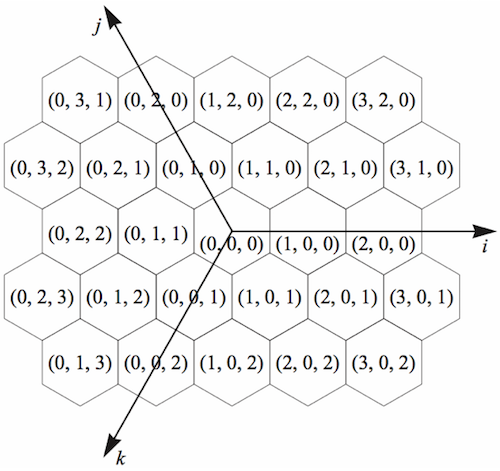
\includegraphics[width=15cm,height=12cm]{ijkp.png}
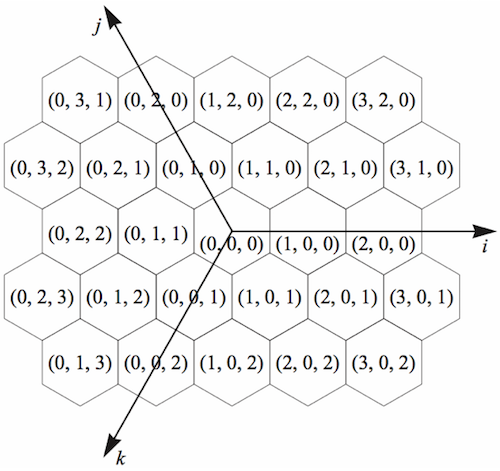
\includegraphics[scale=0.4]{ijkp.png}
\caption{Map Sample with One Possible \textit{ijk} Coordinate System} % 标题
\end {figure}

\newpage
\subsubsection{Notations Based on the \textit{ijk} coordinate system}
% Notations
The notations used in this paper are listed as follows:
\begin{table}[h]
    \centering
    \caption{Notations used in model construction}
    \vspace{3pt}
    \begin{tabular}{>{\centering\arraybackslash}p{6em}>{\centering\arraybackslash}p{30em}}
        \toprule % 绘制第1条线
        Notation         & Meaning                                 \\
        \midrule % 绘制第2条线
        $M
        (i,t)$           & Location of the $i$-th drone
        \uppercase\expandafter{\romannumeral1} at time $t$         \\
        $R
        (j,t)$           & Location of the $j$-th drone
        \uppercase\expandafter{\romannumeral2} at time $t$         \\
        $h
        (x,y,z)$         & Elevation of the point $(x,y,z)$        \\
        $S
        (x,y,z)$         & Fire history of the point $(x,y,z)$
        in the passed $5$ years                                    \\
        $a_i
        (x,y,z)$         & Fire history of the point $(x,y,z)$
        in the $2020-i$-th year,
        $i\in [1,5] \cap \mathbb{N} $                              \\
        $F(x,y,z) $      & Vegetation and urbanizing
        condition of the point$(x,y,z)$                            \\
        $Str(i,x,y,z,t)$ & Signal strength of the
        $i$-th drone at point $(x,y,z)$ at time $t$                \\
        $E
        (x,y,z,N)$       & Supervisory density of the
        point $(x,y,z)$ when there are $N$ drones in the field     \\
        $Slope
        (x,y,z)$         & Maximum slope of the point $(x,y,z)$    \\
        $\gamma$         & Factor related to the weight
        of slope in causing bushfire                               \\
        $\beta
        (x,y,z)$         & Weight of slope in causing bushfire     \\
        $\omega
        (x,y,z)$         & Decreasing rate of signal
        at point $(x,y,z)$                                         \\
        $\alpha$         & Factor related to the weight
        of elevation in causing bushfire                           \\
        $Chg
        (q,x,y,z)$       & Location of the $q$-th charging station \\
        $V_{\text{max}}$ & Maximum flying velocity of a drone      \\
        $N_{\text{SSA}}$ & Amount of drone
        \uppercase\expandafter{\romannumeral1}                     \\
        $N_{\text{rep}}$ & Amount of drones
        \uppercase\expandafter{\romannumeral2}                     \\
        $PF$             & Power consumption for a flying drone    \\
        $PH$             & Power consumption for a hovering drone  \\
        $t_{\text{fl}}
        (t,l)$           & Flight time of the $l$-th drone
        until time $t$                                             \\
        $t_{\text{hov}}
        (t,l)$           & Hovering time of the $l$-th drone
        until time $t$                                             \\
        $T$              & Duration of a day (i.e. $T=1440 \min$)  \\
        $t$              & Current time                            \\
        $Br$             & Total battery power of a drone          \\
        $Ini$            & Location of the EOC                     \\
        \bottomrule % 绘制第3条线
    \end{tabular}
\end{table}

\section{Model Construction}
%%%%%%%%%%%%%%%%%%%%%%%%%%%%%%%%%%%%%%%
%% Model Construction
\subsection{Risk Assessment: Bushfire Risk Model}
% M1
Bushfire risk model measures the probability of catching bushfire for locations in Victoria.
\subsubsection{Applying \textit{ijk} Coordinate System}
%%% coordinate system
To simplify the problem, we do hexagonal paving on the map.
Each of the hexagon is 22.6 km in length.
In addition, We consider the effective area of radio wave signals sent by UAVs to be a spherical area of 20 km radius. Each segment is evaluated from 4 perspectives:
\begin{itemize}
    \item Density of forest coverage,
    \item Elevation,
    \item Slope,
    \item Fire history,
\end{itemize}

The listed items above have impacts on two things:
\begin{itemize}
    \item The possibility of catching fire;
    \item The propagation of radio wave signal.
\end{itemize}

\subsubsection{Vegetation and Other Ground Facilities}\label{BRM-model-vegetation}
%%% M1F1
According to Dissing and Verbyla (2003) \cite{Dorte-lightning01}, thermal circulations triggered by the heating difference among distinct types of vegetation results in a higher probability for a lightning strike to occur. However, a later research based in the State of Victoria (Kilinc and Beringer 2006) claims, that the type and the  density of vegetation in Southern Australia have little impact on the occurrence rate of lightning \cite{Musa-lightning02}. The major cause of lightning there is the homogeneity of forests.

Besides, the leafage has a significant impact on the reflection property of radio wave, which plays an important part in the propagation process.
Several different researches have estimated the decreasing rate of radio wave in various situations. Basing on these results, we consider the state have three types of region: forests, plain, cities. Then we estimated the decreasing factor and valid zone for the radio signal distinctively.

Since the given signals' frequencies are considerably high, it is difficult for the signal to bypass the high-rise barriers like skyscrapers and mountains.
When the drones are passing through the plain, energy loss is little, as the signal only passes through the atmosphere. Under this condition, the radius of the signal's valid zone reaches it's maximum of 20 km. However, high obstacles diminished the zone and the radius reaches it's minimum of 5 km when passing the urban areas. When flying or hovering in the forest regions, the ground signal from front-line personnel's devices and the aerial signal from other drones act differently. According to the experiments of Y.S. Meng.et.al (2010) \cite{Ng-vhf-radio}, when the signal is launched in woods, the signal strength decreases linearly with the frequency of radio wave, and distance (Y. S. Meng.et.al 2009 \cite{Ng-vhfuhf-ieee}).

In the model of Meng's team, the foliage loss in forest region is defined by the equation below:
\begin{equation}\label{ldb}
    L({\rm dB})\cong 0.48 f^{0.43} d^{0.13}
\end{equation}

Considering the drone-to-drone signal propagation, we simply omit the influence of trees, for it is reasonable for flying vehicles to stay above the forests. According to Meng, the background noise is around -75 dBm, so the signal is considered to be undetectable if its strength is lower than -70 dBm. It indicates that when the strength loss is over 18 dB, the point would be regarded as an inaccessible point. Applying Equation \eqref{ldb} to the data we have, it could be verified that the decreasing coefficient for different area are as the equations below:
\begin{equation}\label{omega-function}
    \overline{\omega}
    (x,y,z)=
    \left\{
    \begin{aligned}
         & \overline{\omega}_{\text{city}}=0.25,  \\
         & \overline{\omega}_{\text{forest}}=0.5, \\
         & \overline{\omega}_{\text{plain}}=1
    \end{aligned}
    \right.
\end{equation}

\subsubsection{Elevation and Slope}
%%% M1F2
As mentioned above, the Mountains often cause radio signal loss. Hence, it is natural to introduce an elevation factor $\alpha$ that can be used to evaluate the impact of elevation on causing bushfires.

Lightning strikes were so related to local elevation and slope that many scholars have been using topographic methods to predict bushfires in mountainous areas \cite{Jiao-wildfire-cn}. Previous researches show that strike density has a great leap when the elevation reaches 800 meters, and then it increases linearly with elevation \cite{Musa-lightning02}. Besides, lightning strikes is more likely to formed in the mountainous areas, comparing to the areas with only one high-rise peak \cite{Jiao-wildfire-cn}.


\subsubsection{Fire History}
%%% M1F3
The burned areas tend to catch fires in the future, according to Musa Kilinc and Jason Beringer \cite{Musa-lightning02}. Because ecological environment has been destroyed in the fire, which results in a low capability of local temperature and low capacity of water. None the less, the coked ground with dark shade will absorb more heat than green forests. All these traits formed a hot dry area which can be easily lighted by strikes.

\subsubsection{Functionizing the state of certain location}
%%% M1-Function
To describe a certain location $(x,y,z)$ in the \textit{ijk} coordinate system, we adopted a series of functions\dots

The elevation of the location is denoted by $h(x,y,z)$ , while its slope is denoted by $Slope(x,y,z)$, which means the maximum slope around one point:
\begin{equation}\label{slope}
    \begin{aligned}
        Slope(x,y,z) & =\max\left\{
        \frac{\lVert
            h(x,y,z)-h(x+m,y+n,z+k)
            \rVert}
        {\lvert m\rvert+\lvert n\rvert+\lvert k\rvert}
        \right\},                            \\
                     & m,n,k\in\{-1, 0, 1\},
    \end{aligned}
\end{equation}

Besides, The unit of $h(x,y,z)$ and $Slope(x,y,z)$ are both meters.
\\
The weight of $Slope(x,y,z)$ in causing bushfires is
\begin{equation}\label{weight of slope}
    \begin{aligned}
        \beta(x,y,z) & =\gamma\cdot \max\left\{
        \frac{
            Slope(x,y,z)-Slope(x+m,y+n,z+k)
        }
        {\lvert m\rvert+\lvert n\rvert+\lvert k\rvert}
        \right\},                                                              \\
                     & \gamma\text{ is a constant, and } m,n,k\in\{-1, 0, 1\},
    \end{aligned}
\end{equation}

The vegetational and urbanizing condition $F(x,y,z)$ is defined as the following equation:
\begin{equation}\label{vegetation}%equ6
    F(x,y,z)=
    \left\{
    \begin{aligned}
         & 1,\qquad (x,y,z)\text{ locates in forests,} \\
         & 0,\qquad \text{otherwise.}
    \end{aligned}
    \right.
\end{equation}

The influence of fire history is quantified by bushfire frequency in the passed 5 years (i.e. 2016-2020) :
%equ.7
\begin{equation}\label{Fire-history}
    \begin{aligned}
        S(x,y,z)=\sum_{i=1}^5 (1+\epsilon)^{\frac{1}{i}}\cdot a_i,\quad a_i=\frac{f_i}{23},
    \end{aligned}
\end{equation}
%!check
Here $f_i$ is the amount of fire cases in the $n-i$-th year.

Then we define a function $V(x,y,z)$ to represent how possible a point will catch fire. It is defined below :
\begin{equation}\label{PossibilityFire}
    \begin{aligned}
        V(x,y,z) =                     & V_1(x,y,z)\cdot V_2(x,y,z), \\
        \text{Note: }\qquad V_1(x,y,z) & = [
        0.58 F(x,y,z)                                                \\
                                       & +\alpha\left(
        h(x,y,z)-800
        \right)\cdot
        \beta\cdot u(h(x,y,z)-800)
        ],                                                           \\
        V_2(x,y,z)                     & =\left[
            1+\frac{\ln \left(1+S\left(x,y,z\right)\right)}{3}
            \right],
    \end{aligned}
\end{equation}

here $u(\delta)$ is the stair function:
\begin{equation}\label{Stair}%{equ.11}
    u(\delta)=
    \left\{
    \begin{aligned}
         & 1,\qquad \delta> 0,    \\
         & 0,\qquad \delta\leq 0.
    \end{aligned}
    \right.
\end{equation}

\subsubsection{Future situation in a decade}
%%% M1-Predict
To predict the changing situation in the next decade, we reevaluate the area in the future with the model above.

Since we do not take extreme events into consideration (severe war, earthquake, tsunami, meteorolite, EI Nino etc.), the landscape and urban constructions will not change much in the next decade.

The only changing factor is the fire history, which was evaluated by Equation \ref{Fire-history}. When assessing the situation in the future, $V(x,y,z)$ should be the possibility of catching bushfires on that year instead. For instance, if $V(x,y,z)>867.35$ holds for sometime in the next decades, it means the possibility of catching bushfires is 95\% .

\subsection{UAV Arrangement: Nervous System Model}
% M2
Widespread bushfires in Southeastern Australia are usually preceded by strong winds, a small-scale burning forests can evolve into destructive fires. To minimize such damage, we feel obliged to set a bushfire monitoring and alarming system. In this section, we would introduce a model imitating the nervous system. This model is aiming to figure out the best arrangement of UAVs.

In our model, drones with thermal imaging cameras and telemetry sensors (denoted as drone \uppercase\expandafter{\romannumeral1}) are send out to petrol around the state, detecting fire outbreaks and sending back images. they are working as sensors of the nervous system. Correspondingly, the drones with radio repeaters (denoted as drone \uppercase\expandafter{\romannumeral2}) act as the ganglion, they receive signals and send them out immediately, the command center is the brain in this system.

Our goal is reached by two steps. The first is to find the best routes for drones\uppercase\expandafter{\romannumeral1}. The following two items can help the monitoring and alarming system react to fire outbreaks in time:
\begin{itemize}
    \item The whole state is within the monitoring system's valid zone;
    \item The places that are more probable to catch fire should be paid more attention to.
\end{itemize}

To further the discussion, two new functions was introduced: first for signal strength, denoted as $Str(i,x,y,z,t)$, and second for average signal density of one point, denoted as $E(x,y,z,t)$:
% equ. 19, 20
\begin{subequations}
    \begin{equation}
        Str(i,x,y,z,t)=u\left(8-\lVert (x,y,z)-M(i,t)\rVert\right),
    \end{equation}
    \begin{equation}
        E(x,y,z,N)=\sum_{i=1}^{N_{\text{SSA}}}\frac{1}{T}\int_{0}^{T}S(i,x,y,z,t)dt,
    \end{equation}
\end{subequations}

In the former discussion, we construct the function \label{PossibilityFire} to evaluate how high the possibility is for a point to catch fire. Here, similarly, we introduce a function $Judge(x, y,z)$ defined as $Judge(x,y,z)=\frac{\eta \cdot E}{V}-1$ to judge whether a point is \textit{safe enough}. By \textit{safe enough} we mean: for any drone \uppercase\expandafter{\romannumeral1}, the possibility to discover a bushfire outbreak immediately is high. Here we set the threshold to be 80\%, i.e. $\lambda_{\text{safe}}=0.8$.

Then we are going to link the two types of drones, as in the nervous system the sensors should be linked to the brain. Follow what we mentioned in previous sections, we omit the signal loss caused by forests. However, we would take the influence of high buildings into consideration. And here we define two kinds of vectors $D_i(t)=[d_{ij}(t)]$ and $Q_j(t)=[b_{jk}(t)]$ to represent the signal paths from sensors to the center. The vectors are defined as below:
%equ 16
\begin{subequations}
    \begin{equation}
        d_{ij}(t)=\left\{
        \begin{aligned}
             & 1, \quad \text{if } 0< \lVert M(i,t)-R(j,t)\rVert< 8, \\
             & 0,\quad \text{otherwise},
        \end{aligned}
        \right.
    \end{equation}
    \begin{equation}
        b_{jk}(t)=\left\{
        \begin{aligned}
             & 1, \quad \text{if } 0< \lVert R(k,t)-R(j,t)\rVert< 8, \\
             & 0,\quad \text{otherwise},
        \end{aligned}
        \right.
    \end{equation}
\end{subequations}

Here $i$ denotes the number of drone \uppercase\expandafter{\romannumeral1}s, while $j$ and $k$ denote the number of drone \uppercase\expandafter{\romannumeral2}s.

To ensure that the command center can react to any outbreaks in time, the signal paths should keep unimpeded at all time. Therefore, the variables are limited by the following inequality constraints:
%equ.17
\begin{subequations}
    \begin{equation}
        \sum_{j=1}^{N_{\text{rep}}}d_{ij}\geq 1, \quad i=1,2,\cdots,N_{\text{SSA}}
    \end{equation}
    \begin{equation}
        \sum_{k=1}^{N_{\text{rep}}}b_{jk}\left\{
        \begin{aligned}
            \geq 1, & \qquad \text{if }\sum_{i=1}^{N_{\text{SSA}}} d_{ij}\geq 1, \\
            \geq 2, & \qquad \text{otherwise},
        \end{aligned}
        \right.
    \end{equation}
\end{subequations}

The last factor considered in this section is the charging strategy of drones. Under assumption 9 (see section \ref{ampt09}), none of our drones would be allowed to go further than the distance they can get back to charging stations before they run out of buttery. These ideas triggered the constraints below:
% equ. 18
\begin{subequations}
    \begin{equation}
        t_{\text{hov}}+t_{\text{fly}}=t-105n,
    \end{equation}
    \begin{equation*}
        \text{Denotion:    }
        k(n, t_{\text{fly}}, t_{\text{hov}}) = n\cdot Br-PF\cdot t_{\text{fly}}-PH\cdot t_{\text{hov}},
    \end{equation*}
    \begin{equation}
        \begin{aligned}
            \qquad\qquad & k(n, t_{\text{fly}}, t_{\text{hov}})
            \geq\frac{\min\left\{\lVert
                M(i,t)-Chg(q)
                \rVert ,q
                \right\}}{
                0.417\cdot V_{\text{max}}
            },
            \ \forall t\forall i,                               \\
                         & k(n, t_{\text{fly}}, t_{\text{hov}})
            \geq\frac{\min\left\{\lVert
                R(j,t)-Chg(q)
                \rVert ,q
                \right\}}{
                0.417\cdot V_{\text{max}}
            },
            \ \forall t\forall j,
        \end{aligned}
    \end{equation}
\end{subequations}

Here $0.417$ is the transformation coefficient between real velocity and grid velocity, and $n$ shows how many times that $i$-th drone went back to any charging station.

% M4
\subsection{Generalization: Drone-Terrain Model}
In the first model, we evaluated the hexagonal segments of region from 4 aspects; In the second model we considered the decreasing rate in different terrains. Now, in this model, it was high time to combine the former two models. In this section, our goal is to figure out the best hovering positions for monitoring fires of different sizes on different terrains.

It is reasonable to assume that the front-line staff teams would never enter a burning forest, thus, the valid zone of radio signal need to cover only the frontier of any fires. A tricky way to maintain the signal path is to keep the drones static. Meanwhile, the drones need to come back when nearly running out of battery. Therefore, in this model, arranging the drones as below might work well:
\begin{itemize}
    \item Drone \uppercase\expandafter{\romannumeral2}s are supposed too keep in touch with the front-line teams;
    \item Drone \uppercase\expandafter{\romannumeral1}s are supposed to monitor and report data from front-line personnel's wearable devices;
    \item All the drones will return to the charging stations as long as any fire spotted, except the ones that are components of the communication network.
\end{itemize}

To satisfy these requirements, we re-calculate the signal strength average signal density as below:
%{equ.23}
\begin{equation}
    Str_{\chi}(i,x,y,z)
    =u\cdot\left[
        \overline{\omega}\cdot 8
        -\lVert
        (x,y,z)-M(i)
        \rVert
        \right],
    \chi=\text{\small\uppercase\expandafter{\romannumeral1}}\text{\small ,}
    \text{\small\uppercase\expandafter{\romannumeral2}}\text{\small ,}
\end{equation}

%{equ.24}
\begin{equation}
    E_{\chi}(x,y,z)
    =\sum_{i=1}^{N}Str_{\chi}(i,x,y,z)
    \chi=\text{\small\uppercase\expandafter{\romannumeral1}}\text{\small ,}
    \text{\small\uppercase\expandafter{\romannumeral2}},
    \chi=\text{\small\uppercase\expandafter{\romannumeral1}}\text{\small ,}
    \text{\small\uppercase\expandafter{\romannumeral2}},
\end{equation}

The signal now is a constant as time changes, for the drones are now static.

We also require that the front-line drones be connected to the command center. This is described by the constraints below:
%equ 16.17
% 16
\begin{subequations}
    \begin{equation}
        d_{ij}(t)=\left\{
        \begin{aligned}
             & 1, \quad \text{if } 0< \lVert M(i,t)-R(j,t)\rVert< 8, \\
             & 0,\quad \text{otherwise},
        \end{aligned}
        \right.
    \end{equation}
    \begin{equation}
        b_{jk}(t)=\left\{
        \begin{aligned}
             & 1, \quad \text{if } 0< \lVert R(k,t)-R(j,t)\rVert< 8, \\
             & 0,\quad \text{otherwise},
        \end{aligned}
        \right.
    \end{equation}
    % 17
    \begin{equation}
        \sum_{j=1}^{N_{\text{rep}}}d_{ij}\geq 1, \quad i=1,2,\cdots,N_{\text{SSA}}
    \end{equation}
    \begin{equation}
        \sum_{k=1}^{N_{\text{rep}}}b_{jk}\left\{
        \begin{aligned}
            \geq 1, & \qquad \text{if }\sum_{i=1}^{N_{\text{SSA}}} d_{ij}\geq 1, \\
            \geq 2, & \qquad \text{otherwise},
        \end{aligned}
        \right.
    \end{equation}
\end{subequations}

\section{Sensitive Analysis}
%%%%%%%%%%%%%%%%%%%%%%%%%%%%%%%%%%%%%%%
%% Sensitive Analysis
\subsection{Sensitivity of parameters}
To construct the above models, several constant parameters were used. Their values are given by us and now listed in the table below.
% tab 1
\begin{table}[h]\label{paratab}
    \centering
    \caption{Parameters and Their Values}
    \vspace{3pt}
    \begin{tabular}{>{\centering\arraybackslash}p{6em}>{\centering\arraybackslash}p{30em}}
        \toprule % 绘制第1条线
        Parameter           & Value                \\
        \midrule % 绘制第2条线
        $\overline{\omega}$ & $0.25/ 0.5/ 1$       \\
        $\gamma$            & $0.58$               \\
        $\epsilon$          & $0.5$                \\
        $\alpha$            & $8.68\times 10^{-6}$ \\
        $\eta$              & $2.35$               \\
        $PF$                & $1.2$                \\
        $PH$                & $1.5$                \\
        \bottomrule % 绘制第3条线
    \end{tabular}
\end{table}

While other parameters are set based on formal experiments and researches, the index $\epsilon$ is artificially given. So here we want to analyze the reliance of our model on the value of $\epsilon$, we use the amount of drones needed to represent the behaviour of models, the results are listed below.

% tab 2
\begin{table}[h]
    \centering
    \caption{The Model's Reliance to the Parameter}
    \vspace{3pt}
    \begin{tabular}{>{\centering\arraybackslash}p{6em}>{\centering\arraybackslash}p{30em}}
        \toprule % 绘制第1条线
        Parameter      & Value{\small
        After rounding}               \\
        \midrule % 绘制第2条线
        $\epsilon=0.3$ & $N=36+96$    \\
        $\epsilon=0.5$ & $N=36+96$    \\
        $\epsilon=0.7$ & $N=37+100$   \\
        \bottomrule % 绘制第3条线
    \end{tabular}
\end{table}

From the table above, we can see that the simulation results of the model have little reliance on the value of $\epsilon$, which means that our model is valid and our conclusion is reasonable.

\section{Conclusion}
%%%%%%%%%%%%%%%%%%%%%%%%%%%%%%%%%%%%%%%
%% Result and Conclusion
%简单描述总结以上模型的模拟结果。
The Bushfire Risk Model was first introduced to quantitize and label the terrain of Victoria with the special \textit{ijk} coordinate system. Then the possibility for any place to catch fire was evaluated, and the future situation was predicted.

Based on the Nervous System Model and safety evaluation principles in Section \ref{BRM-model-vegetation}, the optimal arrangement was attained. According to the program simulation, the best choice is to use \textbf{36 SSAs and 96 Repeaters}.

When fires are spotted by the monitoring system, UAVs will be directed as follow:
\begin{itemize}
    \item Drones with SSA that are close to the fire will be sent immediately to keep the area on fire covered by signal.
    \item Drones with repeaters will form the communication web.
    \item Except the necessary drones, other drones will be send back to charge and stand by.
\end{itemize}

Besides, The optimal positions of hover drones are depending on different regions. In our research, three locations are taken into consideration, which is Harieteville (forests of high elevation), Melbourne (urban area), and a place between Omeo and Orbost (plain). The hovering positions are shown in the graphs below.
%{gra.1} {gra.2} {gra.3}
\begin {figure}[h]
\centering % 居中显示
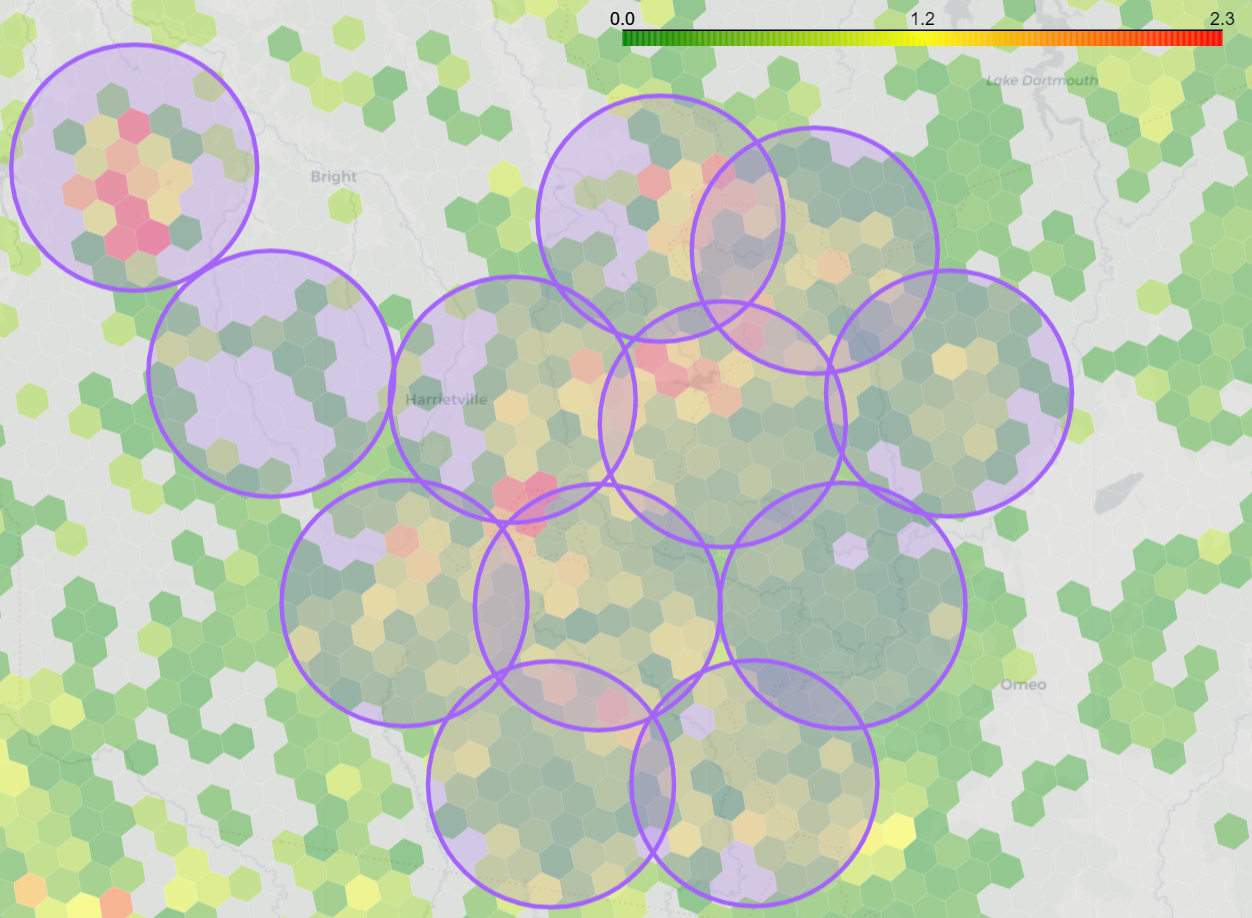
\includegraphics[scale=0.41]{forest.png}
\caption{Forests of Elevation $> 800$ meters} % 标题
\end {figure}

\begin {figure}[h]
\centering % 居中显示
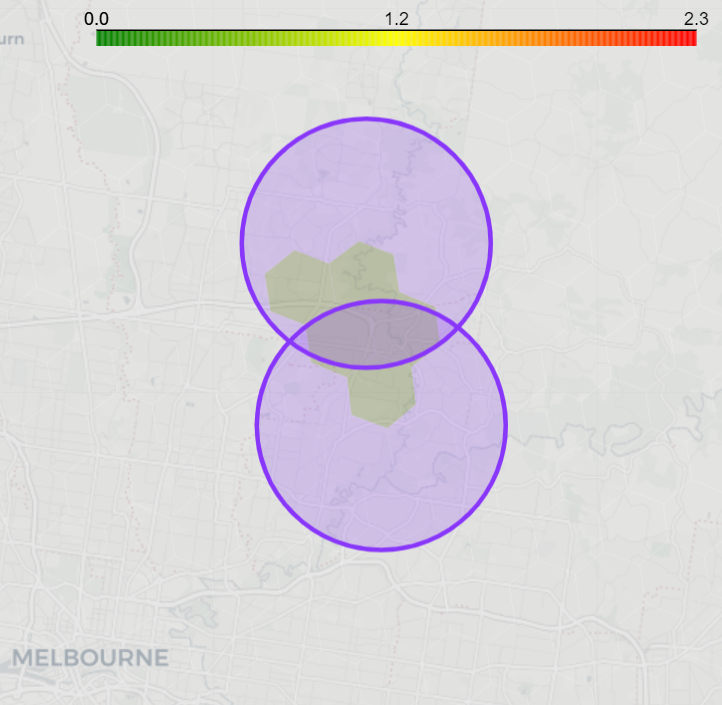
\includegraphics[scale=0.45]{urban.png}
\caption{Urban Area} % 标题
\end {figure}

\begin {figure}[h]
\centering % 居中显示
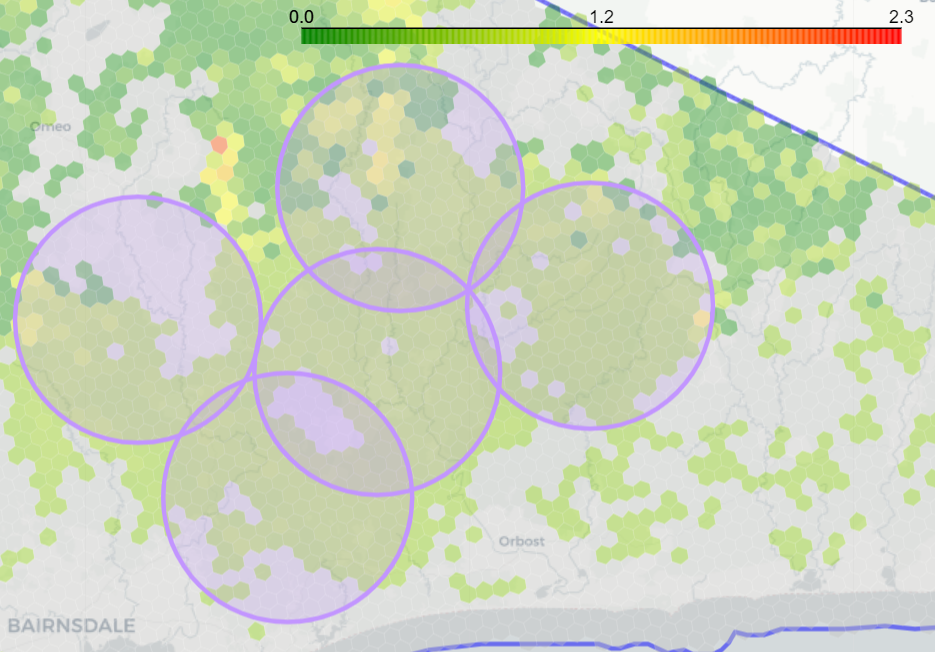
\includegraphics[scale=0.45]{plain.png}
\caption{Plain Area} % 标题
\end {figure}
\FloatBarrier
The changing likelihood of fire events over the next decade in our model was partly illustrated below:

%{gra4},{gra5},
\begin {figure}[h]
\centering % 居中显示
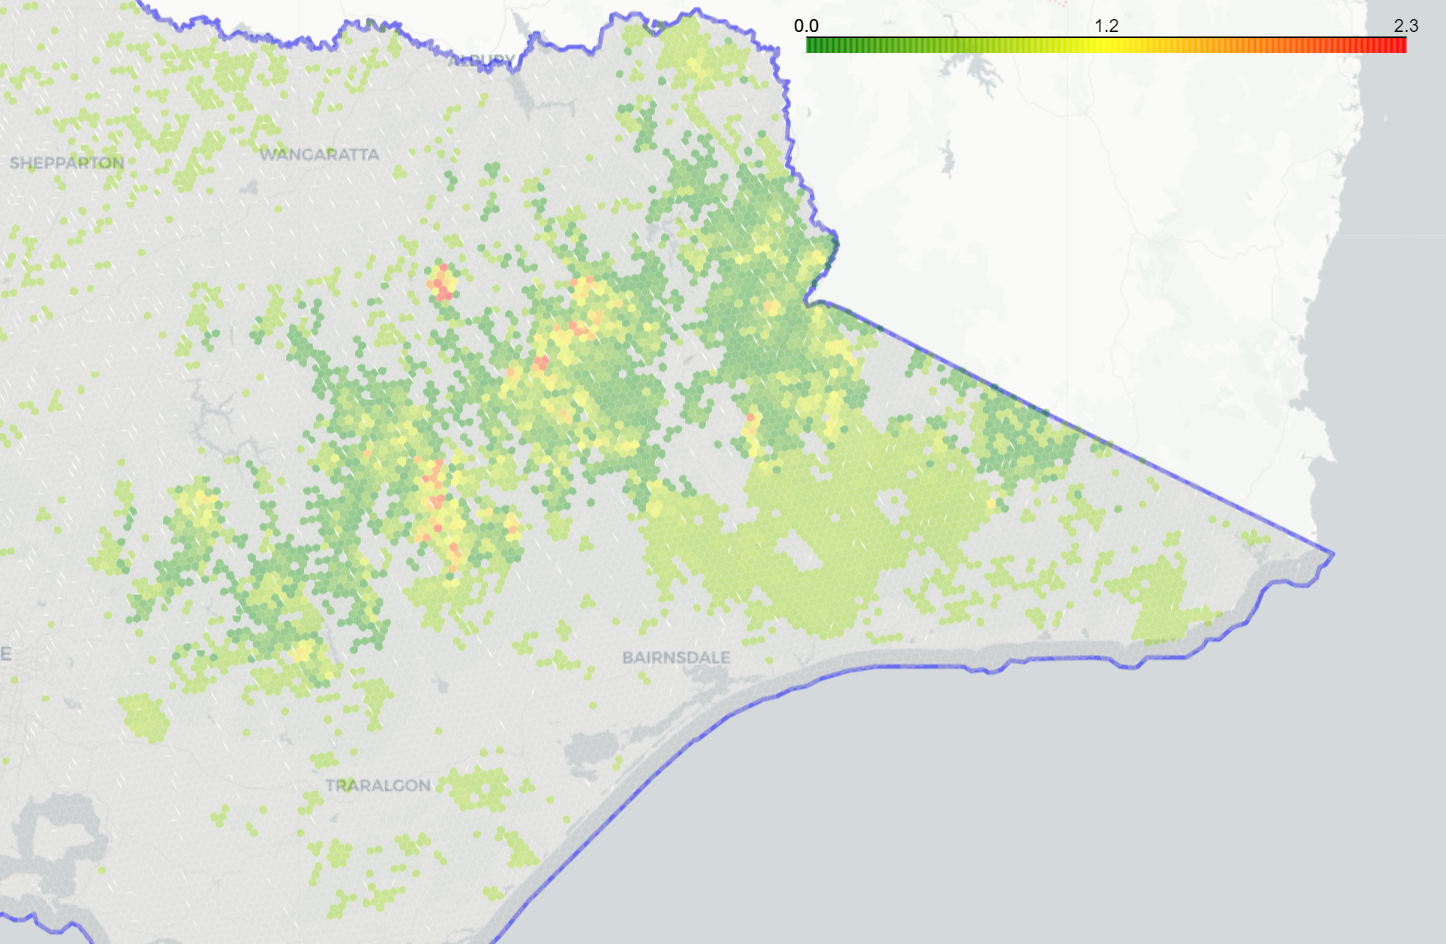
\includegraphics[scale=0.4]{2021.png}
\caption{Condition at 2020} % 标题
\end {figure}

%{gra4},{gra5},
\begin {figure}[h]
\centering % 居中显示
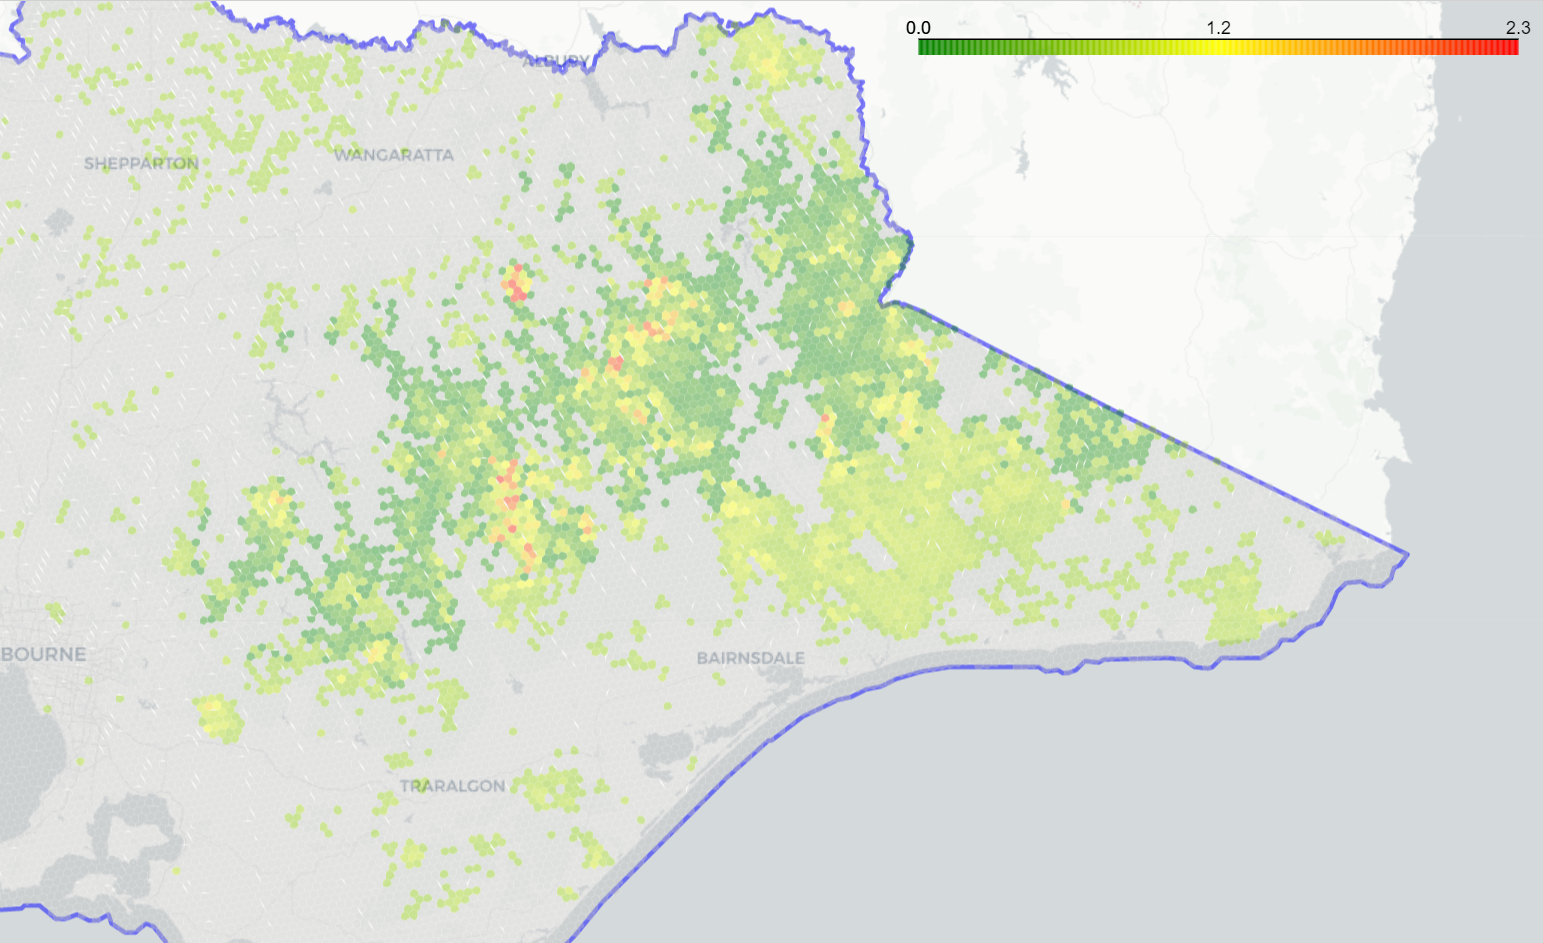
\includegraphics[scale=0.4]{2031.png}
\caption{Condition at 2030} % 标题
\end {figure}

We predict that if the likelihood for huge fires rise the cost on radio repeaters and thermal cameras will rise since they will be put into a hot environment constantly, which rise their risk of breaking. Electricity bills and labour cost will rise, because more people is needed to direct the drones system and drones should charge more frequently.

%%%%%%%%%%%%%%%%%%%%%%%%%%Budget Request页%%%%%%%%%%%%%%%%%%%%%%%%%%
\newpage
\thispagestyle{empty}
\section*{\centering \textbf{Budget Request}}\addcontentsline{toc}{section}{Budget Request}
% 开始写 budget request
\vspace{10pt}
% 基本信息
\begin{flushleft}
    {\small
        \noindent \textsc{Project Name}: Equipment Procurement for Rapid Bushfire Response
        \\ \noindent \textsc{Date Submitted}: February 8th, 2021}
\end{flushleft}
\vspace{10pt}
%\hrule
% explanation
This Budget Proposal provides necessary costs associated with the above named project (the "Equipment Procurement for Rapid") which we would like to pursue . Costs for the Project have been itemized in this Budget Proposal below and justification has been provided for each cost element. Should you have any questions related to this Budget Proposal, please do not hesitate to contact the undersigned.
% request正文
\paragraph{PROJECT DESCRIPTION\\} The state of Victoria has a long history of bushfires, which causing life loss and property damage of varying sizes every year. In the recent years, with advances in technology, we have the opportunity to further reduce the impact of bushfires in Victoria. To better protect lives, interests, and the ecosystem of the state, a new division of \textbf{CFA}, named as \textsc{Rapid Bushfire Response}, would be intended to found, which would aiming at responding quickly to bushfires.

\paragraph{PROJECT PURPOSE\\} In order to equip the proposed new division, it was necessary to build a effective and sensitive monitoring system for bushfires, which could strongly assist the front-line personnel in the daily work of bushfires management. Thus, \textbf{CFA} need the budget to purchase SSA drones and Radio Repeater drones for the monitoring.

\paragraph{COST ELEMENT AND SUMMARY\\}
The following are necessary cost elements of the Project:
\begin{table*}
    \centering
    \begin{tabular}{>{\centering\arraybackslash}p{6em}>{\centering\arraybackslash}p{5em}>{\centering\arraybackslash}p{5em}>{\centering\arraybackslash}p{7em}}
        \toprule
        \textsc{Item Name}
                    & \textsc{Quantity}
                    & \textsc{Unit Price}
                    & \textsc{Extended Price}
        \\ \midrule
        UVA(s)      & $40$                    & $\$ 1, 000$ & $\$ 40, 000$  \\
        Repeater(s) & $100$                   & $\$ 1, 000$ & $\$ 100, 000$ \\
        \bottomrule
    \end{tabular}
\end{table*}

\begin{table*}[h]
    \centering
    \vspace{3pt}
    \begin{tabular}{>{\centering\arraybackslash}p{15em}>{\centering\arraybackslash}p{20em}}
        \toprule % 绘制第1条线
        \textsc{Item Name}                  & \textsc{Total Estimated Cost} \\
        \midrule % 绘制第2条线
        Drones {\small (including 2 types)} & $\$140, 000$                  \\
        \bottomrule % 绘制第3条线
    \end{tabular}
\end{table*}

\FloatBarrier
This budget was developed by \textbf{CFA} of Victoria with adequate modeling that supported this estimate. By the signature below,  we hereby certify that this Budget Proposal reflects the best estimate of the true and necessary costs for the Project, and the information provided herein is accurate, complete and current as of the date of the signature below.

% 清理页眉页脚
\thispagestyle{empty}
% 落款
\vspace{10pt}
\begin{flushleft}
    Country Fire Authority, VIC Australia\\
    {[First Name][Last Name]}\\
    {[Titile]}
\end{flushleft}

\newpage
\section*{References}\addcontentsline{toc}{section}{References}
%%%%%%%%%%%%%%%%%%%%%%%%%%参考文献%%%%%%%%%%%%%%%%%%%%%%%%%%
% 因为不输出此部分到目录 \addcontentsline{}{}{}是添加此标题到目录
\fancyhf{}
\fancyhead[R]{ }
\fancyhead[L]{ }
\bibliography{books}
\Large
\bibliographystyle{IEEEtran}

\end{document}